\chapter{Related work}
\fxnote{Write about Cloud optimized Geotiff somewhere}
\fxnote{Write about gdal2tiles parallelly}

This is not the first project attempting to visualising large raster datasets in an interactive way. It is also not the first attempt at visualizing this particular dataset. 

\fxnote{Write about Sarahs stuff here}

\section{Tilebased raster visualisation}

This is not the first project to follow many of these core concepts. In Bernhard Baumrocks master thesis, he created a webmap, where raster tiles were being colored locally. \citep{Buamrocks}
\begin{figure} [H]
	\centering
	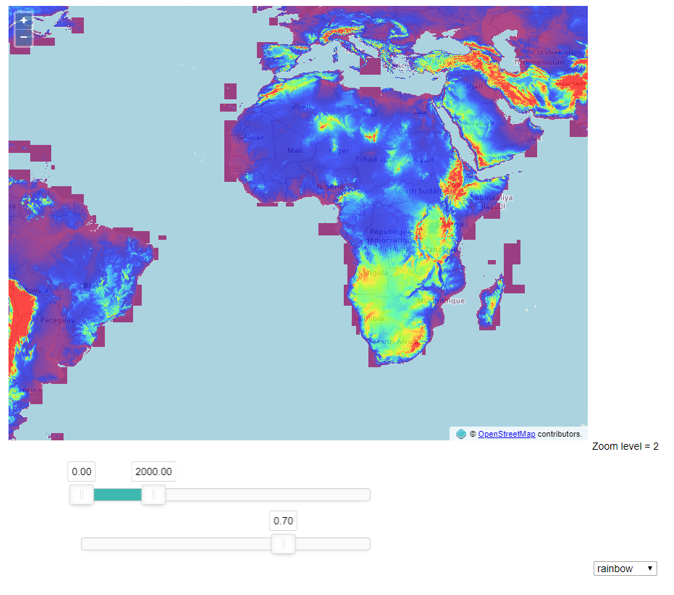
\includegraphics[width=.8\textwidth]{Pictures/BaumrockMap1}
	\caption{The map created by Bernhard Baumrock}
	\label{BaumrockMap1}
\end{figure}

A picture of one of his maps can be seen in figure \ref{BaumrockMap1}. This particular map is not included in his thesis, but it is the most similar to this project. The map shows an unspecified dataset colored in rainbow colors. Below the map are two sliders and a dropdown list with the label “rainbow”. Changing the value in this dropdown list allows the user to switch to another color scheme. The bottom slider is controlling the opacity for the raster layer. The upper slider controls which maximum and minimum values the coloring should be based on. How the map change, when changing the values in the upper slider can be seen in figure \ref{BaumrockMap2}. When zooming in another more detailed layer gets loaded and rendered.
\begin{figure} [H]
	\centering
	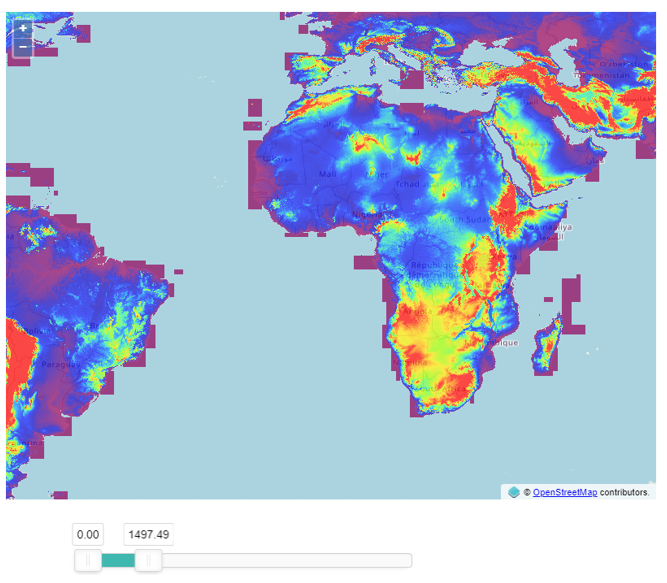
\includegraphics[width=.8\textwidth]{Pictures/BaumrockMap2}
	\caption{How the map change, when using the slider}
	\label{BaumrockMap2}
\end{figure}


%http://webportals.ipsl.jussieu.fr/ScientificApps/dev/forge_patrick/eox/map_01.html

When taking a closer look at the source code it can be seen that the raster is being loaded as tiff tiles with a bit depth of 16 bit. \citep{BuamrocksSouce} Only tiles the currently are visible are being requested unless the tile already have been requested. \citep{Buamrocks}

When comparing with the core concepts for this project, Baumrocks map fulfil most of the criteria. It is locally visualizing only the necessary data. The core concept related to bit depth is relevant in the creation of the tiles, so it does not really apply to this. 
It is also to some extent allowing the user to color the layer based on the current extent. The user can adjust the maximum and minimum values but does not know what the maximum values are in the current extent. 
How the tool functions from a technical perspective is further detailed in section x.

\section{Sections to be written here} 

Other ways of trying to visualizing large rasters:

\begin{itemize}
	\item qgis
	\item makeCitywebsite?
%	\item Visualing with bokeh or folium 
\end{itemize}

Benchmarking using google lighthouse